\section*{Экспериментальная установка}
\begin{figure}[h!]
        \noindent\centering{
            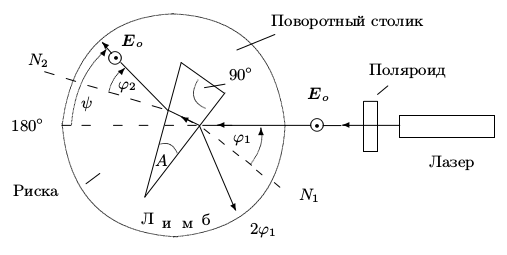
\includegraphics[height = 4cm]{019.png}
        }
        \caption{Схема экспериментальной установки}
    \end{figure}
    Источником излучения служит Не—Nе-лазер
($\lambda = 0,63$ мкм). \\
Угол падения $\varphi_1$ определяется по положению луча, отражённого от передней (входной) грани призмы (рис. 3). Из рис. 2 можно получить
связь углов $\varphi_1, \varphi_2$:
\[\varphi_2 = A + \psi - \varphi_1 ,\]
а угол $\psi$ — отклонение преломлённого луча от первоначального направления — определяется по разности отсчётов на лимбе между точками, куда попадает луч в отсутствие призмы, и точкой, куда попадает преломлённый луч.